%%%%%%%%%%%%%%%%%%%%%%%%%%%%%%%%%%%%%%%%%%%%%%%%%%%%%%%%%%%%%%%%
%%                                                            %%
%%   essentialsOfLatin, Italian translation 2017              %%
%%                                                            %%
%% From:  Henry C. Pearson, Essentials Of Latin For Beginners %%
%%        (1915, New York, American Book Company)             %%
%%                                                            %%
%%    https://archive.org/details/essentialslatin04peargoog   %%
%%                                                            %%
%% Translated by g.p.ciceri <gp.ciceri@gmail.com>             %%
%% ---------------------------------------------------------- %%
%% This translation is Licensed under                         %%
%% Creative Commons Attribution-ShareAlike 4.0 International  %%
%% https://creativecommons.org/licenses/by-sa/4.0/            %%
%%                                                            %%
%%%%%%%%%%%%%%%%%%%%%%%%%%%%%%%%%%%%%%%%%%%%%%%%%%%%%%%%%%%%%%%%

% āēīōū
% ăĕĭŏŭ




\documentclass[nols]{tufte-handout}

%\geometry{showframe} % display margins for debugging page layout

\usepackage{fontspec}
\usepackage{ifxetex}
\setmainfont[Path=./fonts/palatino-linotype/, ItalicFont=palai.ttf, BoldFont=palab.ttf]{pala.ttf}


% \defaultfontfeatures{Mapping=tex-text}
% \setromanfont[Path=./fonts/TeX-Gyre-Schola/,Mapping=tex-text]{TeX Gyre Schola}
% \setsansfont[Path=./fonts/TeX-Gyre-Heros/,Scale=MatchLowercase,Mapping=tex-text]{TeX Gyre Heros}
% \setmonofont[Path=./fonts/TeX-Gyre-Cursor/,Scale=MatchLowercase]{TeX Gyre Cursor}

\usepackage{lipsum}
\usepackage{url}
\usepackage{longtable}
\usepackage{stackengine}

\usepackage{graphicx} % allow embedded images
  \setkeys{Gin}{width=\linewidth,totalheight=\textheight,keepaspectratio}
  \graphicspath{{graphics/}} % set of paths to search for images
\usepackage{amsmath}  % extended mathematics
\usepackage{booktabs} % book-quality tables
\usepackage{units}    % non-stacked fractions and better unit spacing
\usepackage{multicol} % multiple column layout facilities
\usepackage{lipsum}   % filler text
\usepackage{fancyvrb} % extended verbatim environments
  \fvset{fontsize=\normalsize}% default font size for fancy-verbatim environments

% Standardize command font styles and environments
\newcommand{\doccmd}[1]{\texttt{\textbackslash#1}}% command name -- adds backslash automatically
\newcommand{\docopt}[1]{\ensuremath{\langle}\textrm{\textit{#1}}\ensuremath{\rangle}}% optional command argument
\newcommand{\docarg}[1]{\textrm{\textit{#1}}}% (required) command argument
\newcommand{\docenv}[1]{\textsf{#1}}% environment name
\newcommand{\docpkg}[1]{\texttt{#1}}% package name
\newcommand{\doccls}[1]{\texttt{#1}}% document class name
\newcommand{\docclsopt}[1]{\texttt{#1}}% document class option name
\newenvironment{docspec}{\begin{quote}\noindent}{\end{quote}}% command specification environment

% concetti morfosintattici
\usepackage{xspace} 
\newcommand{\noun}{\textsc{sostantivo}\xspace}
\newcommand{\nouns}{\textsc{sostantivi}\xspace}
\newcommand{\adject}{\textsc{aggettivo}\xspace}
\newcommand{\adjects}{\textsc{aggettivi}\xspace}
\newcommand{\gnumber}{\textsc{numero}\xspace}
\newcommand{\gnumbers}{\textsc{numeri}\xspace}
\newcommand{\gender}{\textsc{genere}\xspace}
\newcommand{\genders}{\textsc{generi}\xspace}
\newcommand{\gcase}{\textsc{caso}\xspace}
\newcommand{\gcases}{\textsc{casi}\xspace}
\newcommand{\tense}{\textsc{tempo}\xspace}
\newcommand{\mood}{\textsc{modo}\xspace}
\newcommand{\gverb}{\textsc{verbo}\xspace}
\newcommand{\gverbs}{\textsc{verbi}\xspace}
\newcommand{\adjective}{\textsc{aggettivo}\xspace}
\newcommand{\nom}{\textsc{nom}\xspace}
\newcommand{\gen}{\textsc{gen}\xspace}
\newcommand{\dat}{\textsc{dat}\xspace}
\newcommand{\acc}{\textsc{acc}\xspace}
\newcommand{\voc}{\textsc{voc}\xspace}
\newcommand{\abl}{\textsc{abl}\xspace}
\newcommand{\gexit}{\textsc{uscita}\xspace}
\newcommand{\gexits}{\textsc{uscite}\xspace}
\newcommand{\declinazione}{\textsc{declinazione}\xspace}
\newcommand{\masc}{\textsc{maschile}\xspace}
\newcommand{\femm}{\textsc{femminile}\xspace}
\newcommand{\neut}{\textsc{neutro}\xspace}

\newcommand{\indic}{\textsc{indicativo}\xspace}
\newcommand{\imper}{\textsc{imperativo}\xspace}
\newcommand{\gcong}{\textsc{congiuntivo}\xspace}
\newcommand{\ott}{\textsc{ottativo}\xspace}
\newcommand{\partic}{\textsc{participio}\xspace}
\newcommand{\infin}{\textsc{infinito}\xspace}

\newcommand{\pres}{\textsc{presente}\xspace}
\newcommand{\imperf}{\textsc{imperfetto}\xspace}
\newcommand{\aor}{\textsc{aoristo}\xspace}
\newcommand{\fut}{\textsc{futuro}\xspace}
\newcommand{\perf}{\textsc{perfetto}\xspace}
\newcommand{\pperf}{\textsc{piuccheperfetto}\xspace}

\newcommand{\sing}{\textsc{singolare}\xspace}
\newcommand{\plur}{\textsc{plurale}\xspace}
\newcommand{\dual}{\textsc{duale}\xspace}

\newcommand{\si}{\textsc{sing}\xspace}
\newcommand{\pl}{\textsc{plur}\xspace}
\newcommand{\du}{\textsc{dual}\xspace}

\newcommand{\att}{\textsc{attivo}\xspace}
\newcommand{\med}{\textsc{medio}\xspace}
\newcommand{\pass}{\textsc{passivo}\xspace}
\newcommand{\medpass}{\textsc{medio-passivo}\xspace}


% italianitudini
\renewcommand{\figurename}{Figura}
\renewcommand{\tablename}{Tabella}
\renewcommand{\contentsname}{Indice}

% fix per un qualche problema
\ifxetex
  \newcommand{\textls}[2][5]{%
    \begingroup\addfontfeatures{LetterSpace=#1}#2\endgroup
  }
  \renewcommand{\allcapsspacing}[1]{\textls[15]{#1}}
  \renewcommand{\smallcapsspacing}[1]{\textls[10]{#1}}
  \renewcommand{\allcaps}[1]{\textls[15]{\MakeTextUppercase{#1}}}
  \renewcommand{\smallcaps}[1]{\smallcapsspacing{\scshape\MakeTextLowercase{#1}}}
  \renewcommand{\textsc}[1]{\smallcapsspacing{\textsmallcaps{#1}}}
\fi

% too many float...
\extrafloats{100}
% āēīōū
% ăĕĭŏŭ

\title{Essentials Of Latin. Elementi di Latino. \newline Lezione VII - Declinazione degli Aggettivi. La Concordanza.}

\author[gpciceri]{a cura di Milagathòs: Milo's help to enjoy humanities.}

\date{10 Febbrajo 2017} % without \date command, current date is supplied


\begin{document}

\hyphenation{co-niu-ga-zio-ne}

\maketitle% this prints the handout title, author, and date

\begin{marginfigure}[-2.5cm]
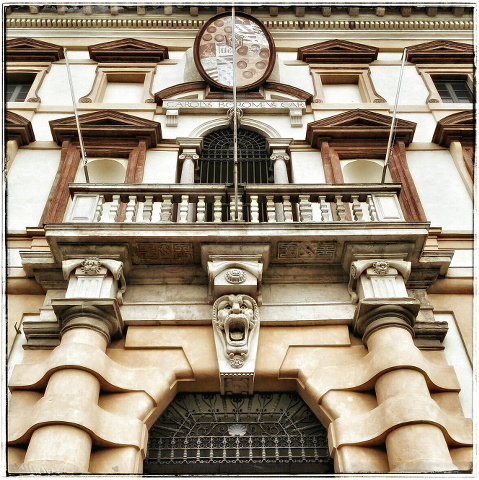
\includegraphics{smallthumb-lesson_I.jpeg}
\setfloatalignment{b}
\end{marginfigure}


\begin{abstract}
\noindent
Queste lezioni riprendono il testo introduttivo al Latino di Pearson\cite{pearson1915}, del quale seguono la numerazione; la struttura di ogni lezione è piuttosto regolare: inizia con \textsc{cenni di morfologia e di sintassi latina}, seguita da un \textsc{piccolo vocabolario} per il lessico; ci sono infine vari \textsc{esercizi} di traduzione e di composizione latina.

\bigskip
\noindent
Lezione VII - Declinazione degli aggettivi della Prima Classe, concordanza dell'aggettivo con il nome a cui si riferisce, vocabolario, esercizi.
\end{abstract}

%\printclassoptions

% āēīōū
% ăĕĭŏŭ

\newthought{62} Gli aggettivi della prima e seconda declinazione \textit{(Prima Classe)} si declinano come i nomi di queste declinazioni. 
Le uscite degli aggettivi maschili e neutri sono come quelle dei nomi della seconda declinazione, 
mentre le uscite degli aggettivi femminili sono come quelle della prima. L'aggettivo guida è \textbf{bonus (a, um)}, \textit{buono}.


\begin{fullwidth}
\begin{table}[!htbp]
  \centering
  \begin{tabular}{l l l l}
    %\toprule
	& \multicolumn{3}{c}{\textsc{Singolare}} \\
	
	& \multicolumn{1}{c}{\textit{maschile}} & \multicolumn{1}{c}{\textit{femminile}} & \multicolumn{1}{c}{\textit{neutro}} \\ 
	
    \nom & bon\textbf{us} & bon\textbf{a} & bon\textbf{um} \\
    \gen & bon\textbf{ī} & bon\textbf{ae} & bon\textbf{ī} \\
    \dat & bon\textbf{ō} & bon\textbf{ae} & bon\textbf{ō} \\
    \acc & bon\textbf{um} & bon\textbf{am} & bon\textbf{um} \\
    \voc & bon\textbf{e} & bon\textbf{a} & bon\textbf{um} \\
    \abl & bon\textbf{ō} & bon\textbf{ā} & bon\textbf{ō} \\
	
	\multicolumn{4}{c}{\textemdash} \\
	
	& \multicolumn{3}{c}{\textsc{Plurale}} \\

    \nom & bon\textbf{ī}  & bon\textbf{ae} & bon\textbf{a} \\
    \gen & bon\textbf{ōrum} & bon\textbf{ārum} & bon\textbf{ōrum}  \\
    \dat & bon\textbf{īs} & bon\textbf{īs} & bon\textbf{īs} \\
    \acc & bon\textbf{ōs} & bon\textbf{ās} & bon\textbf{a}  \\
    \voc & bon\textbf{ī} & bon\textbf{ae} & bon\textbf{a}  \\
    \abl & bon\textbf{īs} & bon\textbf{īs} & bon\textbf{īs}  \\
	
    %\bottomrule
  \end{tabular}
  %\caption[bottom]{Prima Declinazione. \textbf{stella, -ae}, f.}
  \label{tab:normaltab}
  %\zsavepos{pos:normaltab}
\end{table}
\end{fullwidth}


\newthought{63. Frasi Modello.} Esamina le seguenti frasi:
\begin{itemize}
\item[\textsc{1.}] \textbf{Amicus est fidus}, \textit{l'amico è fedele}.  
\item[\textsc{2.}] \textbf{Agricolae sunt validi}, \textit{gli agricoltori sono forti}.  
\item[\textsc{3.}] \textbf{Puellae sunt parvae}, \textit{le ragazze sono piccole}.  
\item[\textsc{4.}] \textbf{Nautas superbos non amamus}, \textit{i marinai orgogliosi non ci piacciono}.  
\end{itemize}
Confronta con cura le uscite dei nomi e degli aggettivi di queste frasi, ed osserva che: \\
\begin{itemize}
\item[\textsc{a.}] Gli aggettivi sono nello stesso \textit{numero, genere, caso} del nome a cui si riferiscono.
\item[\textsc{b.}] Le uscite dei nomi e degli aggettivi correlati non sono sempre uguali: un aggettivo riferito ad un nome mascile della prima declinazione deve avere le uscite maschili, quelle della seconda declinazione. Trova l'esempio che illustra questa regola.
\end{itemize}

\newthought{64. Esercizio.} Declina assieme \textbf{nauta bonus}, \textit{il buon marinaio};  
\textbf{poculum magnum}, \textit{la grande coppa};
\textbf{agricola validus}, \textit{il forte agricoltore}.

\newthought{65. Regola di Sintassi.} Concordanza dell'aggettivo. L'aggettivo concorda con il nome cui si riferisce in numero, genere e caso.

\newthought{66. Vocabolario} 

\begin{multicols}{2}
    \noindent \hangindent=1em \textbf{malus, a, um}, agg., \textit{cattivo, malvagio}.  \\
    \noindent \hangindent=1em \textbf{magnus, a, um}, agg., \textit{grande}.  \\
    \noindent \hangindent=1em \textbf{parvus, a, um}, agg., \textit{piccolo}.  \\
    \noindent \hangindent=1em \textbf{meus, a, um}, agg., \textit{mio}.  \\
    \noindent \hangindent=1em \textbf{tuus, a, um}, agg., \textit{tuo}.  \\
    \noindent \hangindent=1em \textbf{gratus, a, um}, agg., \textit{gradito, piacevole}.  \\
    \noindent \hangindent=1em \textbf{albus, a, um}, agg., \textit{bianco}.  \\
    \noindent \hangindent=1em \textbf{carus, a, um}, agg., \textit{caro}.  \\
    \noindent \hangindent=1em \textbf{peritus, a, um}, agg., \textit{esperto}.  \\
    \noindent \hangindent=1em \textbf{longus, a, um}, agg., \textit{lungo}.  \\
    \noindent \hangindent=1em \textbf{latus, a, um}, agg., \textit{largo, ampio}.  \\
    \noindent \hangindent=1em \textbf{novus, a, um}, agg., \textit{nuovo}.  \\
    \noindent \hangindent=1em \textbf{fidus, a, um}, agg., \textit{fedele, leale}.  \\
    \noindent \hangindent=1em \textbf{superbus, a, um}, agg., \textit{orgoglioso}.  \\
    \noindent \hangindent=1em \textbf{validus, a, um}, agg., \textit{forte, robusto}.  \\

	\noindent \hangindent=1em \textbf{convocō}, v., \textit{io chiamo a raccolta, io convoco}.  \\
	\noindent \hangindent=1em \textbf{hodie}, avv., \textit{oggi}.  \\
	\noindent \hangindent=1em \textbf{nunc}, avv., \textit{ora}.  \\
	
\end{multicols}
% āēīōū
% ăĕĭŏŭ

\newthought{67. Esercizi di Ripasso}
\\
\textsc{I.} \quad
\textsc{1.}~Filiae equis cibum dant. \quad
\textsc{2.}~Inopia pecuniae Marco agricolae non est grata. \quad
\textsc{3.}~Vocatisne incolas Galliae? \quad
\textsc{4.}~Ubi Romani pugnant? \quad
\textsc{5.}~Nautae reginae dona grata dant. \quad
\textsc{6.}~Nauta Marco agricolae bonum vinum dat.
\\
\textsc{II.} \quad
\textsc{1.}~Il marinaio da doni graditi a (sua) figlia. \quad
\textsc{2.}~La figlia di Marco, l'agricoltore, è in città. \quad
\textsc{3.}~Essi danno soldi alle donne. \quad
\textsc{4.}~Egli porta grano in città.


\newthought{68. Esercizi}
\\
\textsc{I.} \quad
\textsc{1.}~Equi albi frumentum in oppidum portant. \quad
\textsc{2.}~Ubi est hodie nauta peritus? \quad
\textsc{3.}~In oppido nunc est nauta. \quad
\textsc{4.}~Dona meis amicis sunt semper grata. \quad
\textsc{5.}~Equum agricolae valido feminae dant. \quad
\textsc{6.}~Regina superba in magnum oppidum servos convocat. \quad
\textsc{7.}~Dominus servos fidos vocat. \quad
\textsc{8.}~Mea filia non est in horto. \quad
\textsc{9.}~Hodie peritos agricolas non culpamus. \quad
\textsc{10.}~Dona reginae incolas fidos delectant. \quad
\textsc{11.}~Est nova luna. \quad
\textsc{12.}~Cur in hortum agricolas validos convocas?
\\
\textsc{II.} \quad
\textsc{1.}~Un marinaio non è sempre fedele. \quad
\textsc{2.}~Essi ora lodano l'esperto agricoltore. \quad
\textsc{3.}~La regina convoca i malvagi abitanti in città. \quad
\textsc{4.}~Oggi lodiamo il tuo amico fedele. \quad
\textsc{5.}~Ci sono abitanti leali in città. \quad
\textsc{6.}~La regina dà a Marco, l'agricoltore, uno schiavo.


\begin{figure}[!b]
  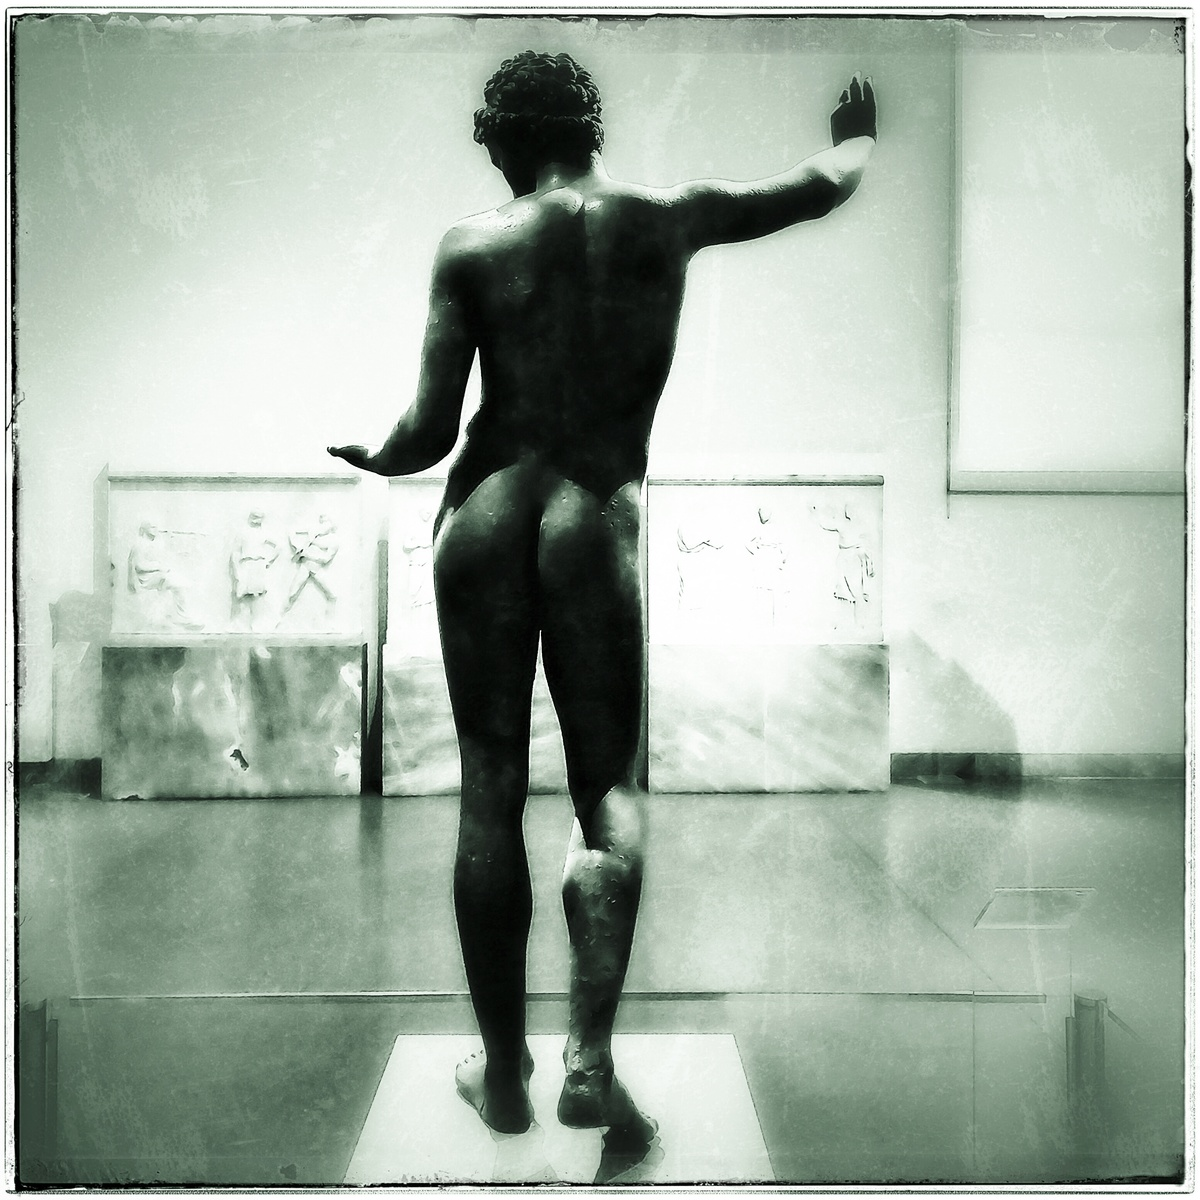
\includegraphics[width=0.8\linewidth]{thumb-lesson_VII.jpeg}
  %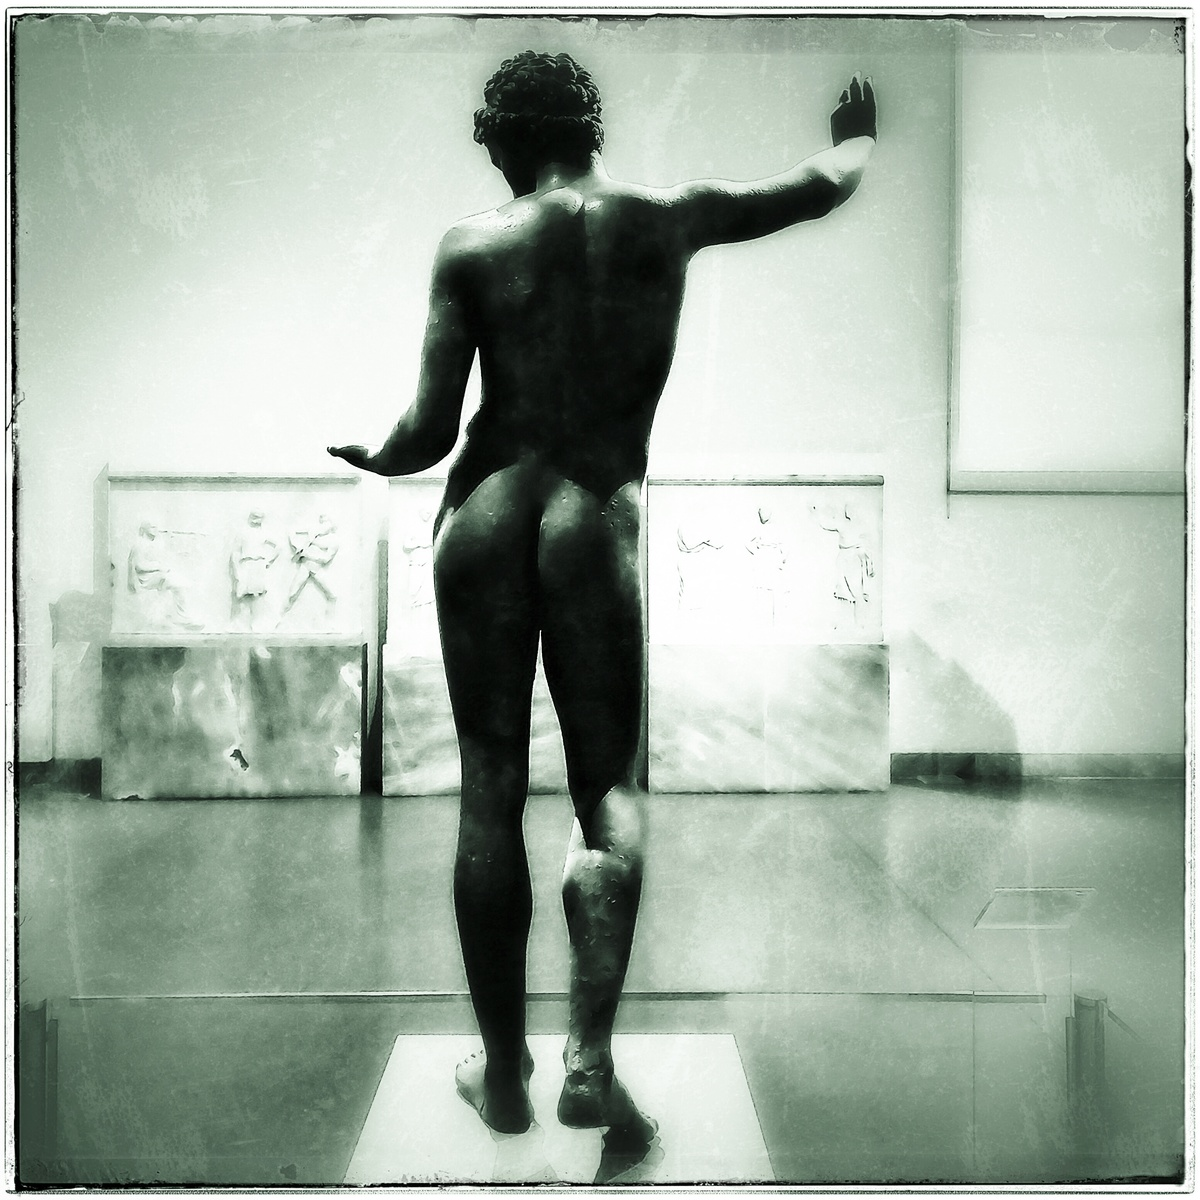
\includegraphics{thumb-lesson_VII.jpeg}
  \caption{Pavia: Almo Collegio Borromeo}
  \label{fig:textfig}
  %\zsavepos{pos:textfig}
  %\setfloatalignment{b}
\end{figure}

 

\nobibliography{latinBiblio}
\bibliographystyle{alpha}


\end{document}
